\documentclass[11pt, oneside]{article}   	% use "amsart" instead of "article" for AMSLaTeX format
\usepackage{geometry}                		% See geometry.pdf to learn the layout options. There are lots.
\geometry{letterpaper}                   		% ... or a4paper or a5paper or ... 
%\geometry{landscape}                		% Activate for for rotated page geometry
%\usepackage[parfill]{parskip}    		% Activate to begin paragraphs with an empty line rather than an indent
\usepackage{graphicx}				% Use pdf, png, jpg, or eps§ with pdflatex; use eps in DVI mode
\usepackage{listings}								% TeX will automatically convert eps --> pdf in pdflatex		
\usepackage{amssymb}

\title{Cubist Data Exercise}
\author{Xinlong Li}
\date{}							% Activate to display a given date or no date

\begin{document}
\maketitle
\section{Problem Description}
%\subsection{}

%    \texttt{df['Signal']}
%    \texttt{df['ClosePrice']}

\


The aim of this data exercise is to test a data source, \texttt{df['Signal']}, which claims to be predictive of future returns of the SP500 index (use SPY as a proxy). There will be two main parts in the following text. The first part performs a data cleaning on the given data-frame $df$, identifying any errors in the data. flagging them , and suggest a corrected value or if advisable, There are also illegal values which are directly deleted. The second part presents a time series analysis to check if \texttt{df['Signal']} could be used to predict future values of \texttt{df['ClosePrice']} from SP500.

There are three columns in the data-frame \texttt{df}. (1)\texttt{df['Date']}. (2)\texttt{df['Signal']}, which may be predictive of future returns of the SP500 index (use SPY as a proxy). (3)  \texttt{df['ClosePrice']},  which is the SPY price.



\section{Data Cleaning}

\

Firstly, we should check if there are missing values. There are 6 missing dates which are actually trading days but are absent in the data-frame. They are
\begin{lstlisting}
	2013-01-14 2013-01-15 2013-01-16 2013-01-17
	2014-01-06 2014-02-11
\end{lstlisting}
The first 4 dates are continuous and we fill them with interpolation. The last 2 dates are single dates and we impute with previous value. We also check if  the dates are unique.

Then we check if all the dates are trading days.  We find  that there are 4 days which are illegal. 
\begin{lstlisting}
	2013-12-25 is Christmas Day
	2014-01-01 is New Year's Day 
	2014-02-08 and 2014-02-09 are weekends
\end{lstlisting}
So we drope them with their corresponding rows.

Next, we check if there are outliers in \texttt{df['Signal']}.
\begin{figure}[htbp]
   \centering
   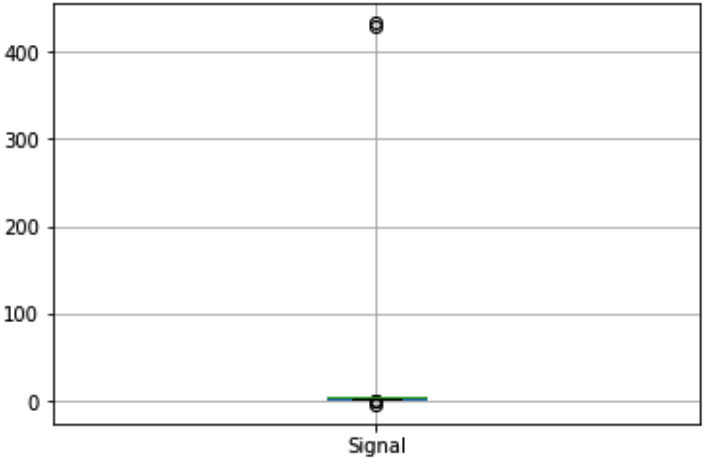
\includegraphics[width = 2.5in]{so1.png} 
    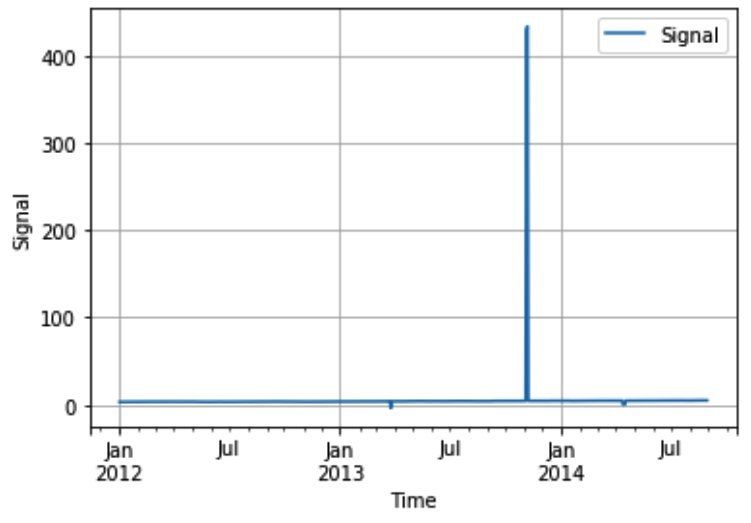
\includegraphics[width = 2.5in]{so2.png}
   \caption{Show outliers at large values. Left: Box-plot of \texttt{df['Signal']}.  Right: \texttt{df['Signal']} vs \texttt{df['Date']}}
   %\label{fig:example}
\end{figure}
From Figure 1, we can see there are 2 data points which are significantly larger than others. They are 
\begin{lstlisting}
	2013-11-05, 2013-11-06
\end{lstlisting}
we  replace them with interpolated values and check again.
\begin{figure}[htbp]
   \centering
   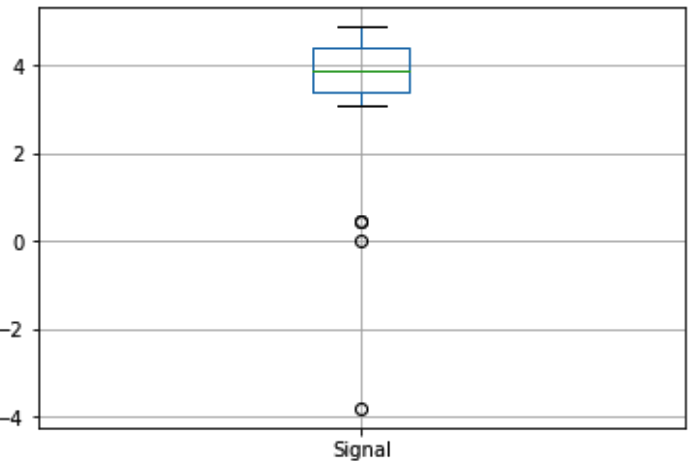
\includegraphics[width = 2.5in]{so3.png} 
    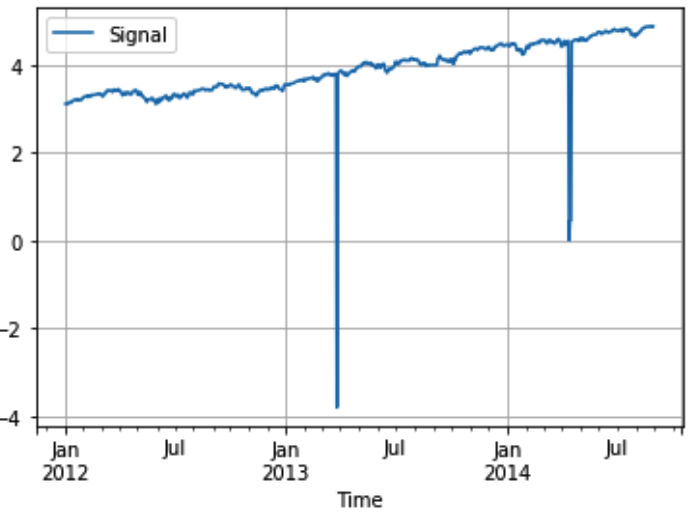
\includegraphics[width = 2.5in]{so4.png}
   \caption{After fixing the outliers at large values.  Show outliers at small values. Left: Box-plot of \texttt{df['Signal']}.  Right: \texttt{df['Signal']} vs \texttt{df['Date']} }
   %\label{fig:example}
\end{figure}
We can see from Figure 2 that there are also a few data points which are significantly smaller than others. They are
\begin{lstlisting}
	2013-03-26
	2014-04-14 2014-04-15 2014-04-16.
\end{lstlisting}
After filling modifying these data points, we perform the same action on \texttt{df['ClosePrice']} and find 3 outliners
\begin{lstlisting}
	2013-09-12 2013-09-13 2013-09-16
\end{lstlisting}

Finally, we can plot \texttt{df['Signal']} and \texttt{df['ClosePrice']}  on top of each other (shown in Figure 3). \texttt{df['ClosePrice']} is approximately 40 times bigger than \texttt{df['Signal']}.
\begin{figure}[htbp]
   \centering
   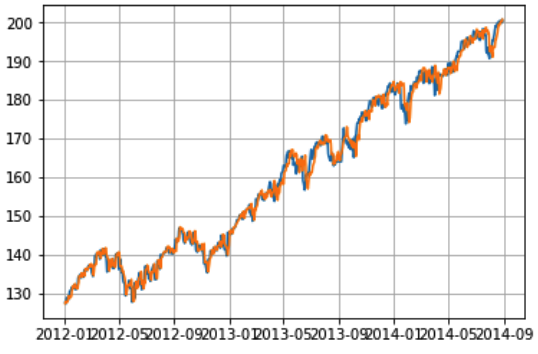
\includegraphics[width = 2.5in]{sc.png} 
       \caption{41$\times$\texttt{df['Signal']} (blue) and \texttt{df['ClosePrice']} (orange) vs \texttt{df['Dates']} after data cleaning.}
   %\label{fig:example}
\end{figure}




\section{Time Series Analysis}

\

Firstly, we have a glance on the decomposition plot of \texttt{df['Signal']}(shown in Figure 4).
\begin{figure}[htbp]
   \centering
   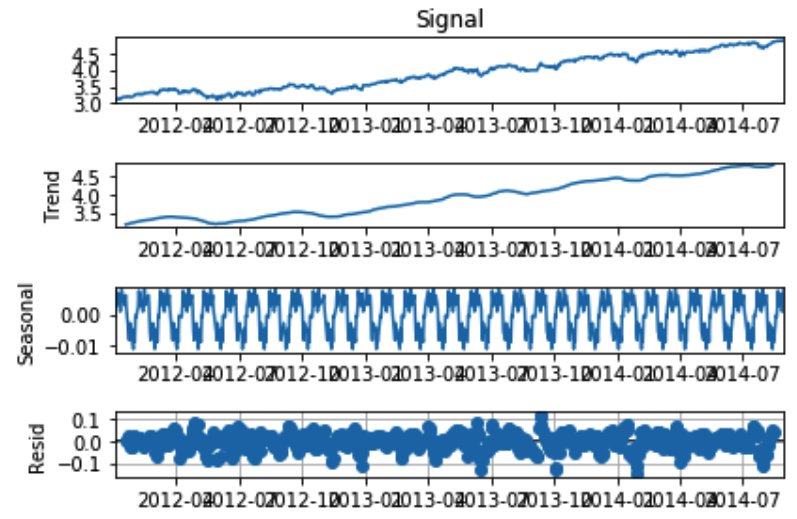
\includegraphics[width = 4in]{decom.png} 
       \caption{Decomposition plot of \texttt{df['Signal']}.}
   %\label{fig:example}
\end{figure}

The amplitude of seasonal curve is quite small. So we ignore the seasonality of time series \texttt{df['Signal']}.

\subsection{Check Stationary}

\

From  Fgure 4 above we can see that the time series is not stationary. We confirm this using Augmented Dickey Fuller (ADF) Test.
\begin{lstlisting}
	Results of ADF Test:
		Test Statistic                  -0.306330
		p-value                          0.924603
		#Lags Used                       2.000000
		Number of Observations Used    666.000000
		Critical Value (1%)             -3.440207
		Critical Value (5%)             -2.865889
		Critical Value (10%)            -2.569086
\end{lstlisting}
The test statistic is bigger than the critical values and the p-value is big, which cannot reject the null hypothesis.   This implies that the time series \texttt{df['Signal']} is not stationary.

Kwiatkowski-Phillips-Schmidt-Shin (KPSS) test also gives the same answer.
\begin{lstlisting}
	Results of KPSS Test:
		Test Statistic            3.241585
		p-value                   0.010000
		Lags Used                20.000000
		Critical Value (10%)      0.347000
		Critical Value (5%)       0.463000
		Critical Value (2.5%)     0.574000
		Critical Value (1%)       0.739000
\end{lstlisting}
With the test statistic bigger than the critical values and p-value smaller than 0.05, we reject the null hypothesis, which confirms again that the time series \texttt{df['Signal']} is not stationary. 

We do a quick differencing on the time series \texttt{df['Signal']}  to make it stationary.
\begin{lstlisting}
	df['Signal_diff'] = df['Signal'] - df['Signal'].shift(1)
	df['Signal_diff'].dropna().plot()
	adf_test(df['Signal_diff'].dropna())
	kpss_test(df['Signal_diff'].dropna())
	
	Results of ADF Test:
	Test Statistic                 -20.202023
	p-value                          0.000000
	#Lags Used                       1.000000
	Number of Observations Used    666.000000
	Critical Value (1%)             -3.440207
	Critical Value (5%)             -2.865889
	Critical Value (10%)            -2.569086
	
	Results of KPSS Test:
	Test Statistic            0.050405
	p-value                   0.100000
	Lags Used                20.000000
	Critical Value (10%)      0.347000
	Critical Value (5%)       0.463000
	Critical Value (2.5%)     0.574000
	Critical Value (1%)       0.739000
\end{lstlisting}

\subsection{ARIMA Model}

\

Let's have a look at the Auto Correlation Function (ACF) figure and Partial Auto Correlation Function (PACF) figure of  \texttt{df['Signal$\_$diff']}  (shown in Figure ).
\begin{figure}[htbp]
   \centering
   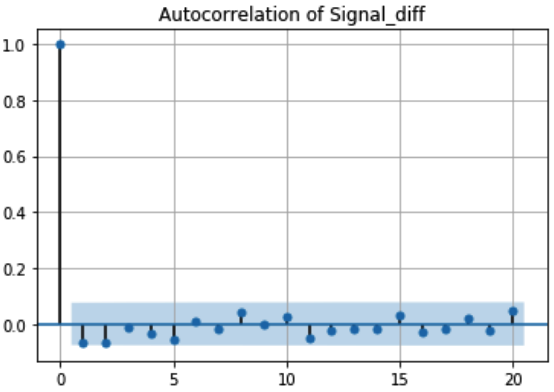
\includegraphics[width = 2.5in]{acfdiff.png} 
    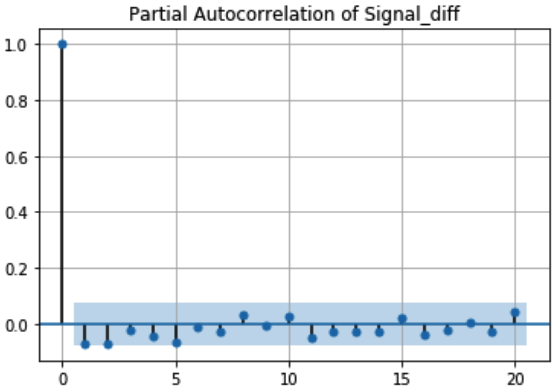
\includegraphics[width = 2.5in]{acfdiff2.png}
   \caption{ ACF and PACF of \texttt{df['Signal$\_$diff']}}
   %\label{fig:example}
\end{figure}

We can conclude that p  and q should be smaller than 2 in ARIMA(p,d,q) Model. We set d = 1 since we did a differencing on the column \texttt{df['Signal']}. In the end, we find that p = q = 1 has lower AIC. So we try (p,d,q) = (1,1,1)
\begin{figure}[htbp]
   \centering
   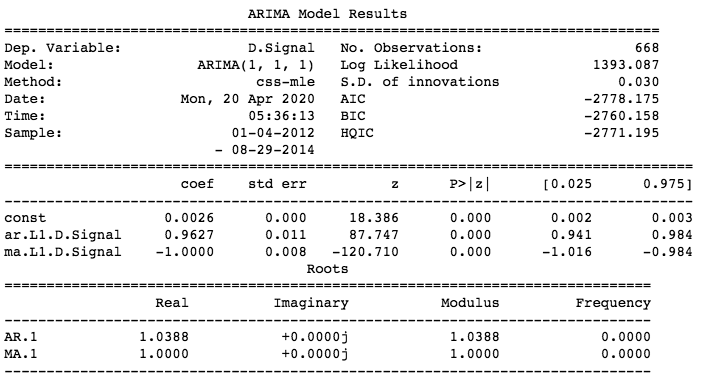
\includegraphics[width = 5in]{amira1.png} 
       \caption{Result of ARIMA(1,1,1) training on \texttt{df['Signal']}}
   %\label{fig:example}
\end{figure}

The result of ARIMA(1,1,1) model is shown in Figure 6. The autoregressive term has a p-value that is less than the significance level of 0.05. So I can conclude that the coefficient for the autoregressive term is statistically significant. The same with moving average term.We also plot the residue in Figure 7. the residues follow the normal distribution. And no significant correlation is present, we can conclude that the residuals are independent. Overall, it seems to be a good fit. \begin{figure}[htbp]
   \centering
   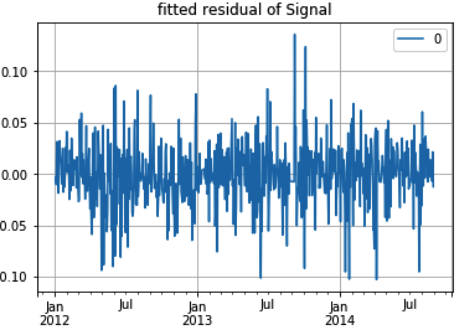
\includegraphics[width = 2.5in]{re1.png} 
    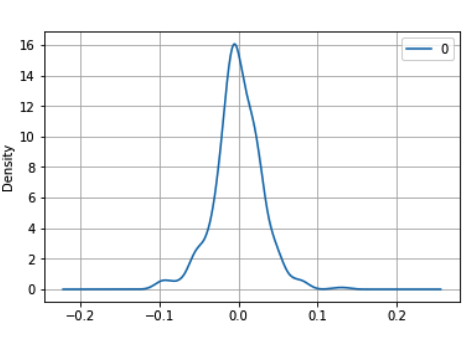
\includegraphics[width = 2.5in]{re2.png}
    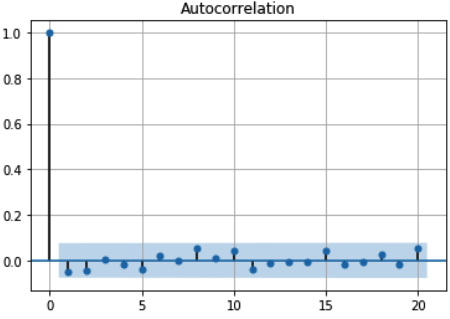
\includegraphics[width = 2.5in]{re3.png}
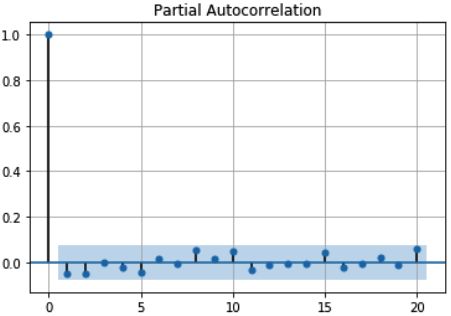
\includegraphics[width = 2.5in]{re4.png}
   \caption{Top left: Residues vs \texttt{df['Date']}.  Top right: distribution of residues. Bottom left: ACF of residues. Bottom right: PACF of residues}
   %\label{fig:example}
\end{figure}

In addition, we can run a Ljung Box Test on the residues and  the square value of residues in ARIMA(1,1,1) model, which gives a p-value of 0.18 and 0.74, respectively. They are both larger than 0.05, which implies our model does not show lack of fit.

We show the  figure of  ARIMA(1,1,1) model fitting \texttt{df['Signal']}.
\begin{figure}[htbp]
   \centering
   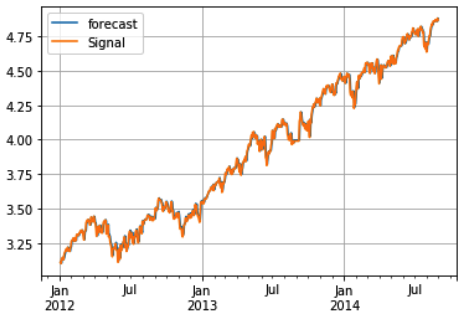
\includegraphics[width = 2.5in]{fitt.png} 
       \caption{\texttt{df['Signal']} curve and its fitting curve.}
   %\label{fig:example}
\end{figure}
Figure 8  shows that the ARIMA(1,1,1) model can fit \texttt{df['Signal']} very well. so let's use it to forecast \texttt{df['ClosePrice']} of SP500 to see if \texttt{df['Signal']} could be predictive of future returns of the SP500 index.

We use the last 100 rows of data-frame \texttt{df} as test set and the rest of the rows as training set. We use \texttt{df['Signal']} of the training set to train the ARIMA(1,1,1) model. Then we  forecast the \texttt{df['ClosePrice']} in the test set using the model. Note that we divided the \texttt{df['ClosePrice']} by 38 to make \texttt{df['ClosePrice']} and \texttt{df['Signal']} equal at the starting date of the test set.
\begin{figure}[htbp]
   \centering
   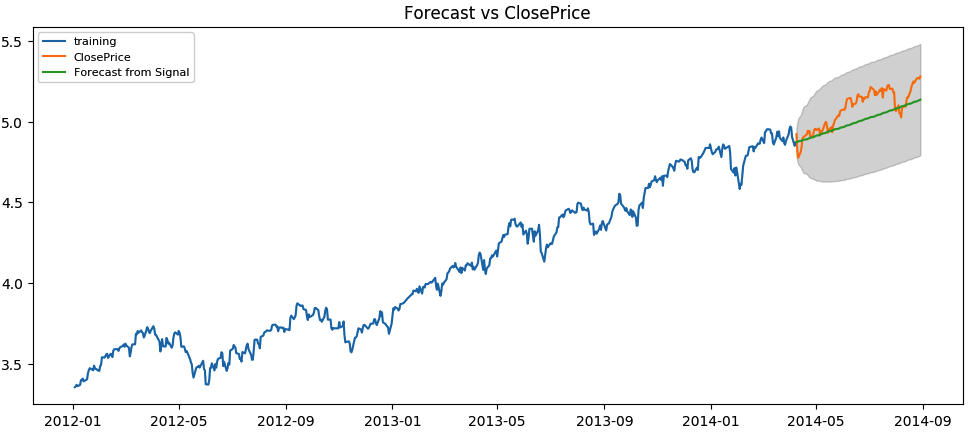
\includegraphics[width = 5in]{fc.png} 
       \caption{Forecasting of future \texttt{df['ClosePrice']} data by training the past \texttt{df['Signal']} data using ARIMA(1,1,1) model. The grey area means 95$\%$ confidence. }
   %\label{fig:example}
\end{figure}
From figure 9, the ARIMA(1,1,1) model seems to give a directionally correct forecast. And the actual observed \texttt{df['ClosePrice']} lies within the 95$\%$ confidence band ($\alpha=0.05$).

In the end, we calculate accuracy metrics in Figure 10. The MAPE, Correlation and Min-Max Error are used to evaluate the forecast. Around 1.7$\%$ MAPE implies the model is about 98.3$\%$ accurate in predicting the next 100 trading days. So I think this forecast is quite good.
\begin{figure}[htbp]
   \centering
   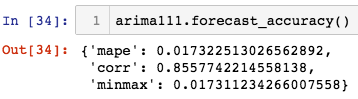
\includegraphics[width = 2.5in]{am.png} 
       \caption{Calculating the accuracy matrices}
   %\label{fig:example}
\end{figure}


\section{Conclusion}

\

From this data exercise, we conduct a time series analysis to test the predictive power of \texttt{df['Signal']}. In the data cleaning part, we find  4 illegal dates which are not trading days, 6 missing dates which are actually trading days but are absent in the data-frame, 6 outliers belonging to \texttt{df['Signal']} and 3 outliers belonging to \texttt{df['ClosePrice']}.

In the time series analysis part. We check the stationary, perform a ARIMA model fitting, analyze the residues and forecast the close price. All of the above shows that \texttt{df['Signal']}  can be predictive of future returns of the SP500 index (use SPY as a proxy).

However, we should tell the Portfolio Manager that \texttt{df['ClosePrice']}. is  APPROXIMATELY 40 times bigger than \texttt{df['Signal']}. We should calculate this factor today before we forecast the close price tomorrow.













\end{document}  